\section{The ICLR claims, revisited}
\label{sec:iclr}

\begin{figure}[t]
  \centering
  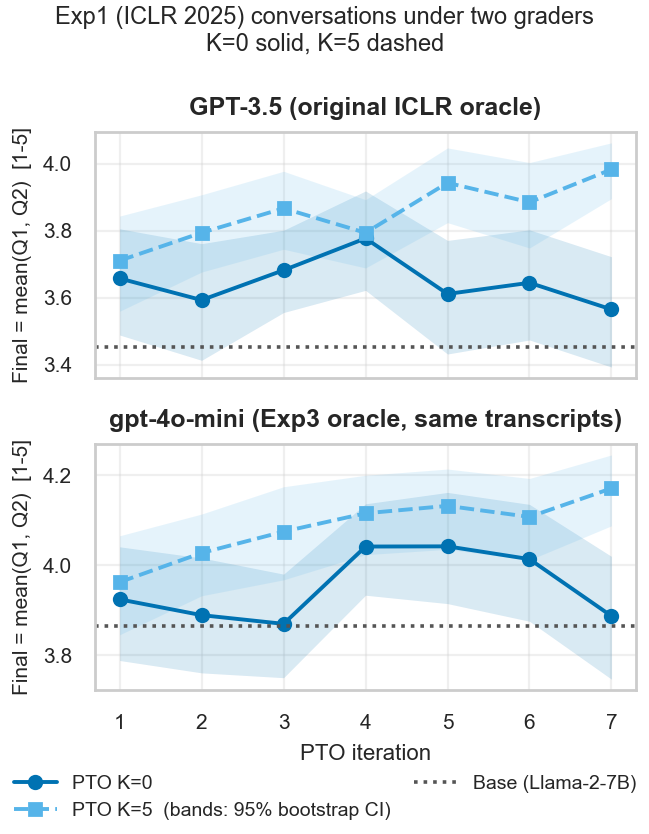
\includegraphics[width=\linewidth]{figures/crossgen_exp1_fig_col.png}
  \caption{The poster's own 1{,}440 conversations (Llama-2-7B, GPT-3.5 patients; PTO, seven
    iterations) under the original GPT-3.5 oracle (top) and re-scored by \primaryjudge{} (bottom).
    \Kz{} solid, \Kf{} dashed, base dotted; 95\% bootstrap CIs of the mean. Separate $y$-axes: the
    new grader reads $0.19$--$0.43$ higher; never averaged.}
  \label{fig:crossgen}
\end{figure}

The poster made three claims for $K{=}5$ over $K{=}0$ \citep{baruch2025pto}: higher reward,
significant only on Q2 and at the post-hoc best iterations; shorter conversations; and the lowest
standard deviation, read as stability. Signs below are $K{=}0$ minus $K{=}5$.

\paragraph{Higher reward: real for its regime, not for this one.} In our experiment the PTO $K$
contrast on the reward (\QQ{}) never significantly favours \Kf{} (\S\ref{sec:reward}). Before
attributing that to the newer grader we re-scored the poster's 1{,}440 conversations with our
training oracle. The ordering
survives: \Kf{} is above \Kz{} at all seven matched iterations under both graders
(Holm-significant at iterations 3 and 7 under \primaryjudge{}, at 5 and 7 under GPT-3.5); at the
arm level --- each conversation's score averaged over an arm's seven iterations, then paired ---
the contrast is $-0.132$ (\dz{} $-0.54$, CI $[-0.180, -0.084]$) under \primaryjudge{} and
$-0.206$ (\dz{} $-0.61$) under GPT-3.5. The poster's best-vs-best comparison (its \Kz{}
iteration~4 against its \Kf{} iteration~7, ``L0\,M4 vs L5\,M7'') is $-0.129$ (\dz{} $-0.25$,
Wilcoxon $p{=}.006$) under the new grader against $-0.206$ (\dz{} $-0.25$, $p{=}.33$, paired-$t$
$p{=}.016$) under the old. The new grader compresses the gap by about a third and does not
remove it (Figure~\ref{fig:crossgen}); our null is a property of what changed between the
experiments (\S\ref{sec:discussion}), not of the judge.

\paragraph{Shorter conversations: reversed for PTO, optimizer-conditional.} The poster reported
L5\,M7 cutting the mean session from $43.7$ to $34.4$ turns. In our experiment every arm ends
shorter than its base, but the $K$ contrast splits by optimizer: at PTO iteration~10 the \Kf{} sessions are
\emph{longer}, $28.70$ vs $20.39$ utterances ($-8.31$, \dz{} $-0.55$, CI $[-11.22, -5.26]$,
$p_{\text{Holm}}{<}.001$), while at GRPO iteration~5 they are shorter, $22.57$ vs $30.68$
($+8.10$, \dz{} $0.53$); \S\ref{sec:mechanism} traces the PTO lengthening to its selection.

\paragraph{Lowest standard deviation: fails, and was a ceiling artefact.} Under the training
oracle PTO \Kf{} is \emph{more} dispersed than \Kz{} on \QQ{} at 10 of 10 iterations (median SD
ratio $1.17$; the persona-paired Pitman--Morgan test is Holm-significant at four iterations,
never the reverse, the unpaired Brown--Forsythe test at none); GRPO shows no dispersion
difference (median ratio $1.04$). The lowest-SD trained
state is a \Kz{} state (PTO \Kz{} iteration~10), and across the 35 trained states SD is almost
a function of the mean --- Spearman$(\text{mean}, \text{SD}) =
-0.87$ on \QQ{} --- because the Cooperative third of personas saturates the 1--5 scale. Under
the held-out judge, which never awards \QQ{} $\geq 4.5$, the PTO arms are indistinguishable in
dispersion (median ratio $1.01$, no Holm-significant iteration; GRPO's one significant row,
iteration~4 with \Kf{} less dispersed, does not hold at iteration~5) and the mean--SD
correlation is $-0.38$. Low SD measured
the ceiling, not the optimizer.
